\section{Iteration No 3: Infrastructure and Interconnect}
\label{sec:iteration_no3}

\subsection{Milestones and Goals}

As has been discussed in the section \Nameref{sec:hpc_infrastructure} the second most important
aspect of a \ac{HPC} system, after the computation is the communication.
As the networking was the glass ceiling of the previous iteration, both in maximal parallel performance
as well as slowing down the communication needed for tightly coupled applications,
the goal of this iteration is to improve the networking of the cluster.


\begin{enumerate}
    \item \textbf{Multi \ac{CNI} Support} The current networking setup of the cluster is based on a simple \textit{Flannel}
          overlay network. In order to support more complex networking setups, the \ac{CNI} needs to be able to support more than one network
          interface at a time. This will allow the cluster to be able to support multiple types of networking interfaces, such as \ac{IB} and Ethernet.
    \item \textbf{Utilizing \ac{IB}} The current cluster includes five nodes that are equipped with InfiniBand (\ac{IB}) networking,
          enabling faster node-to-node communication, which is crucial for \ac{HPC} as detailed in sections \ref{sec:suggarch_network} and \ref{sec:networking_interconnects}.
          This allows the \ac{IB}-enabled nodes to communicate with each other using \ac{IB} while maintaining the capability to interact with the rest
          of the cluster over standard networking protocols, ensuring seamless integration within the existing infrastructure.
\end{enumerate}
\subsection{Implementation}


\subsubsection{Multi \ac{CNI} Support}

The first step in achieving multi \ac{CNI} support was to identify a \ac{CNI} that supports multiple interfaces.
As described in the section \Nameref{sec:K8sNetworking}, the way Kubernetes handles networking is by creating a
\ac{VETH} for each pod, which gets patched into the  \ac{CNI} plugin.
Therefore, if a pod is to have multiple network interfaces, this needs to be handled by the \ac{CNI} plugin.
One such \ac{CNI} plugin is \textit{Multus}, which acts as a meta-plugin, allowing multiple other \ac{CNI} plugins to
plug into a single pod, providing multiple network interfaces.
This is achieved by acting as an intermediary between the host and the container, providing a single interface to the kubelet{kubelet}, while
plugging into multiple \ac{CNI} other plugins to provide the necessary networking interfaces to the container\footcite{multusK8snetworkplumbingwgMultuscni2024a}.

\pagebreak

\begin{figure}[!ht]
    \vspace{0.8cm}
    \centering
    \scalebox{0.35}{
        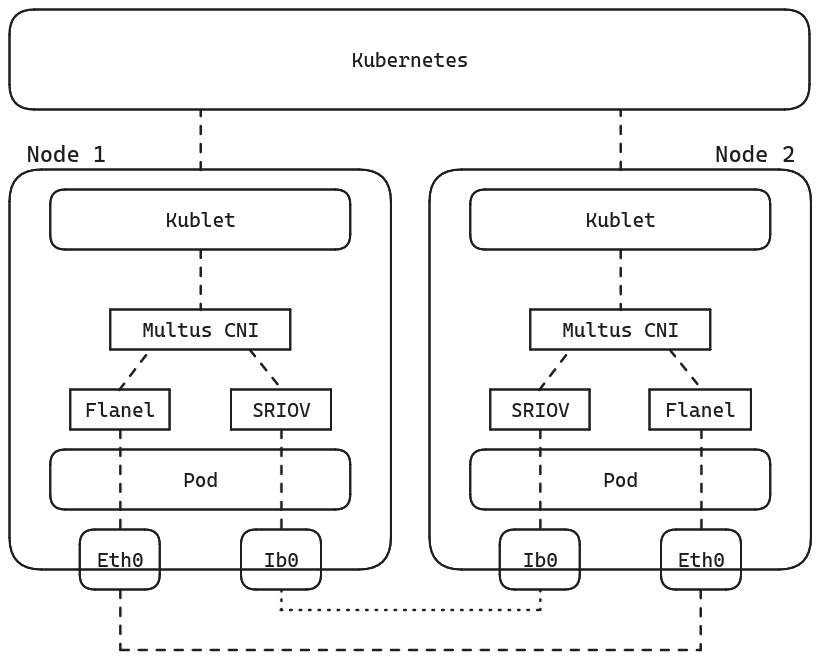
\includegraphics{./graphics/Multus.png}
    }
    \caption{Multus \ac{CNI} with SRIOV and Flannel\protect\footnotemark}
    \label{fig:multus_cni}
\end{figure}
\footnotetext{Based on: \cite{redhatMakingHighPerformance}}



In diagram \ref{fig:multus_cni}, above one can see the end goal of this whole iteration, as this
diagram shows how \textit{Multus} slots itself between the \textit{kublet} and the default \ac{CNI} plugin ,
in hour case \textit{Flannel}, and then plugs in another \ac{CNI} plugin, in this case \textit{SRIOV}
being used to provide the direct access to the \ac{IB} network.

To implement this, the nodes were first \gls{cordoned} and \gls{drained} to ensure that no pods were running on them.
The binaries for \textit{Multus} were compiled and builtd into a container image, which was run as a daemonsets on the cluster.
The container placing accessing the filesystem of the hosts, copying over the binaries, and most importantly
replace the config files of the previous \ac{CNI} plugin and not deleting but deprioritizing them\footcite{multusK8snetworkplumbingwgMultuscni2024a}.
This is done so the \textit{Multus} plugin will be the first to be called by the \textit{kubelet},
when creating a pod; if nothing else is defined the \textit{Multus} plugin will then simply call the default \ac{CNI} plugin,
in this case \textit{Flannel}.

Generally, installing another \ac{CNI} plugin would not be much more complicated as the \textit{Multus} plugin.
Adding the \ac{CNI} binary to all hosts and adding a generic configuration file to the \textit{kubelet} would be enough.
However, as the goal is to connect an \ac{IB} network to the pods, the process is a bit more complicated and will be discussed in the next section.

\pagebreak
\subsection{Evaluation of Results}

Installing the \textit{Multus} plugin was successful, and the plugin was able to run as expected.
Injecting itself automatically between the existing \textit{Flannel} plugin and the \textit{kubelet} worked exactly as expected.


\subsubsection{Utilizing \ac{IB}}

As described in the chapters \Nameref{sec:hpc_infrastructure} and in the design of this prototype \Nameref{sec:suggarch_network},
the Interconnect is a crucial part of a \ac{HPC} system.
Especially so in in \ac{GASNet} systems relying on the low cost \ac{RDMA} based injections to achieve its
global address space (further discussed in \ref{sec:gasnet}).

But Infiniband is by far not as deeply integrated in the Kubernetes ecosystem as the generic \ac{TCP/IP} stack.
As such the process of connecting the \ac{IB} network to the pods is a bit more complicated than just installing a \ac{CNI} plugin.

First the \ac{IB} network needs to be configured and available on the hosts.
The right kernel modules need to be loaded, the right firmware installed and the right \ac{UEFI} settings need to be set.
If all the hardware is set up correctly, and the network has a subnet manager running, the \ac{IB} network should be available on the hosts.

Unlike the \ac{TCP/IP} stack on Kubernetes the \ac{IB} network is not made out emulated
interfaces within the Pod which get routed by the containerized infrastructure until it funnels
out a single interface on the host (as described in \ref{sec:K8sNetworking}).
Instead, the \ac{IB} network is a physical network that
which needs to execute these operations on the hardware level in order to maintain the
extremely low latency and high bandwidth that \ac{IB} networks are known for\footcite{pfisterIntroductionInfiniBandArchitecturea}.

But in order to provide more than one container at a time with isolated access to the \ac{IB} network,
the \ac{IB} network needs to somehow be split up into multiple virtual interfaces for the pods to use.
As this has already been a topic of interest to virtualization technologies, wanting to take
advantage of the low latency and high bandwidth of \ac{IB} networks similar to the pass through
solutions described in the section \Nameref{sec:virtualization}.

\text{SRIOV}:

One such technology is \ac{SRIOV}, which splits a single physical \ac{PCI} into multiple virtual \ac{PCI} interfaces,
which can then be access by different entities on the host, acting as if they were physical interfaces.
These \ac{VF}s can be configured by directly accessing the original \ac{PF} to create the \ac{VF}s as needed.

Both of these still reside in the hosts' kernel space and are not yet available to the pods.
So if a \ac{VF} has been created manually the Pod needs a way to access this \ac{VF} directly.
This is where the \textit{ib-sriov-cni} comes in, as it is a simple \ac{CNI} plugin
that allows a pod to connect to an existing \ac{VF} on the host\footcite{ib-sriov-cni-repoK8snetworkplumbingwgIbsriovcniInfiniBand}.
While this plugin offers access to a \ac{VF} it needs to be
provided with all necessary network information to establish the connection.
This includes everything, from the \ac{PCI} address of the \ac{VF} to access to the \ac{IPAM}
data of the network the \ac{VF} should connect to.
This requires setting up and writing the configuration for each pod on each node manually.
The \textit{ib-sriov-cni} plugin itself simply resides as a binary in the \textit{CNI} directory of the host,
being called upon if \textit{Multus} is instructed to use it for a pod.


\text{SRIOV-Device-Plugin}:

In order to avoid to manually configuring the network data for each pod,
the \textit{SRIOV-Device-Plugin} can be used.
This Kubernetes plugin scans the nodes via a Daemonset for \ac{PCI}
devices which match a given definition and index them.
This creates a resource pool of \ac{SRIOV} devices available to connect to,
which can then be used by the \textit{ib-sriov-cni} plugin to connect to the \ac{VF}s.
Reducing the need to manually declare the data of the \ac{PCI} device manually for each pod.
This needs to be configured with the parameters of the
\ac{PCI} devices to be matched and then run as a Daemonset on the cluster.



\text{Sriov-Network-Operator}:

Now that the pod can automatically discover \ac{VF}s on the host,
the network data configuration for the pods need to be set up,
so that a pod can actually receive the configuration of which network to connect to.
The \textit{sriov-network-operator} is a Kubernetes operator that allows a user to define
a custom resource that describes the desired state of the network configuration of the cluster.
Requesting a specific network devices to provide the necessary \ac{VF}s to the pods.

Once the \textit{sriov-network-operator} pod has been deployed to the head node of the cluster,
it will start a daemon on each node which keeps track of the state of each node and the network
devices ready to be used by the \textit{ib-sriov-cni} plugin. It also sets up endpoints
for the KubernetesAPI to interact with the \textit{sriov-device-plugin}.

Once a user creates an instance of the custom resource called \textit{SriovNetworkNodePolicy},
the \textit{sriov-network-operator} will create a \textit{NetworkAttachmentDefinition} object
which will can be referenced in the pod configuration as an annotation.
While in the background the \textit{sriov-device-plugin} on the nodes register the difference between
desired and actual state of the network devices, and signals the KubernetesAPI to update the state of the
Node. The Api then calls on the \textit{sriov-network-operator} to update the configuration.


Once the \ac{VF}s are available a pod can be created with only the name of
the network to connect to, the once a pod with the right keyword is requested, the
resource injector matches the network name with the existing \textit{NetworkAttachmentDefinition}
and injects the necessary information into the pod configuration.
Using this configuration the \textit{Multus} plugin then knows to call the \textit{ib-sriov-cni} plugin
providing the injected network information to the pod.


\begin{figure}[!ht]
    \vspace{0.8cm}
    \centering
    \scalebox{0.35}{
        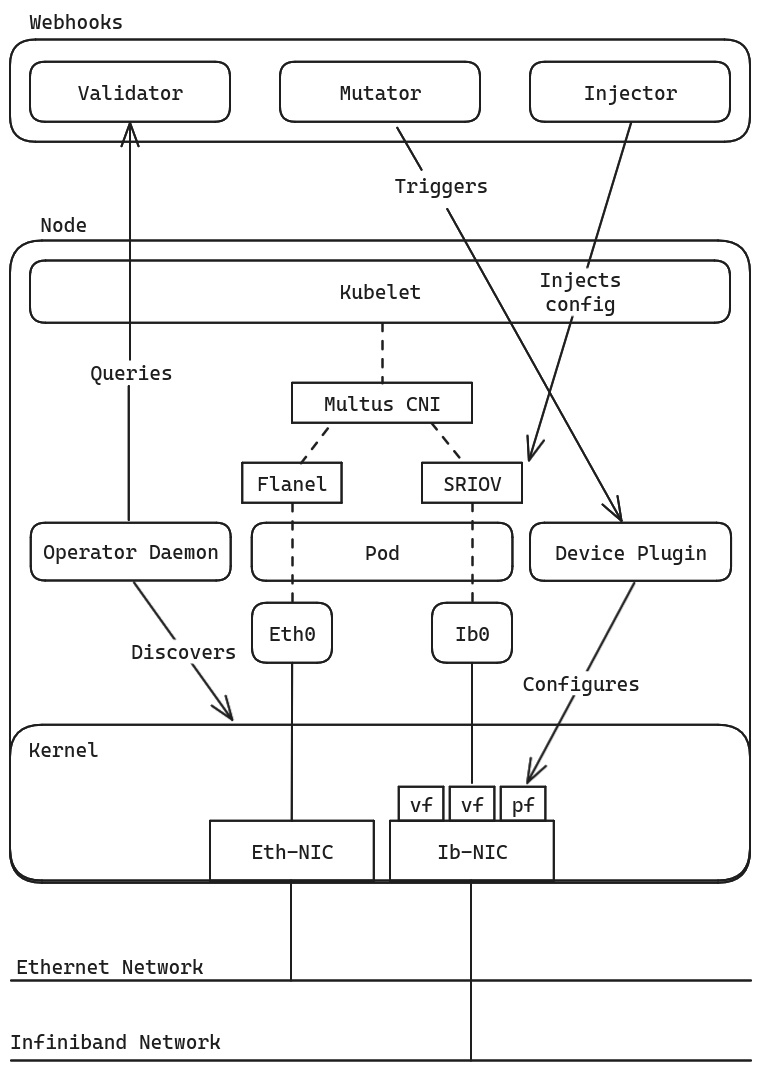
\includegraphics{./graphics/SRIOV Infrasturcture.png}
    }
    \caption{Simpliefied architecture of a SRIOV enabled Kubernetes Node}
    \label{fig:Sriov_infrastructure}
\end{figure}

In diagram \ref{fig:Sriov_infrastructure} above, a simplified version of the interactions within a single node of the cluster is shown.
Not pictured are the daemons running on the head node or, calls of the Kubernetes API, or the mutating
config maps which are being mutated by the system to declare the current and desired states of the network devices.

\textbf{Implementation process}

During the implementation of this iteration many problems arose in orchestrating these many interdependent components.
As the use case for \ac{IB} enabled \ac{HPC} on Kubernetes has not been widely explored, many of the components
are originally intended for other use cases, unmaintained or proprietary. A large part of the existing documentation
was addressed at fellow developers, describing the necessary steps built the components, but do not
provide information about how to deploy or configure them, as this is assumed to be known by the developer of the
component in the first place. This made the process of setting up the \ac{IB} network on the cluster a very
time-consuming and painstaking process, involving a lot of reverse engineering and trial and error, sometimes
discovering known caveats documented only as a side note in the source code of the component.
The most helpful resource was \textit{Redhat}s documentation\footcite{redhat-openshiftSingleRootVirtualization} for their \textit{OpenShift} platform,
their custom Kubernetes based platform. While useful and detailed, their documentation is only targeted
at their platform and the translation to vanilla Kubernetes is not always straightforward.

Amongst the issues encountered was a communication problem, between the Kubernetes API and the
sriov-operator-webhook-config \textit{mutatingwebhookconfigurations} and its \textit{validatingwebhookconfigurations}.
While the webhook was configured according to the documentation, the underlying pod was able to receive
and log requests and the provided certificates were valid, signed and concurrent between the webhook and the container
the API was getting a "500 Internal Server Error - Bad Gateway" when trying to reach the webhook. This behavior
could not be reproduced in any other way during debugging.
While the issue was worked around at first by overwriting the webhook, it was later coincidentally discovered that
The system requires the filename of the certificate file to be identical to the secret containing the file.
While a banal issue, it was only documented in form as a comment in the code of the webhook itself\footcite{sriov-network-operator-repoSriovnetworkoperatorBindataMaster}.

The most Significant hurdle was the in transparent configuration of the \ac{IB} device and the components directly
interacting with it. As there is little community effort behind these projects and numerous proprietary
components involved, the configuration of the \ac{IB} device was the part of the prototyping process which
cased the project to hit the deadline for the prototyping process, requiring the project to be continued
after release of this paper.

\textbf{Current State}

While the above described infrastructure has been set up and brought to a working state,
completely enabling the configuration of the cluster by declaring the required configuration of the
nodes and declaring a network. Even the mounting of the \ac{IB} network to the pods has been achieved.
And while the \ac{VF} functions are accessible and intractable by the pods, the pods are not able to
able to send or receive data over the \ac{IB} network.
This is due to the interface requiring the \ac{RDMA} module requiring to be set to the \textit{"exclusive mode"}.
While setting the device to exclusive mode is a simple command, this in turn disables the \ac{VF}s completely.
While this is most likely a trivial configuration issue, the deadline of the prototyping process has been reached
and this paper is to be handed in. The project will be continued after the release of this paper.
The current state of the project can be found in the corresponding repository and will be updated as
the project progresses\footcite{joneckerthBachelorsThesisProjectMain}.

\subsection{Conclusion}

While the setup of the infrastructure as a whole was successful within on the Kubernetes Level,
the many small issues resulted in the project running out of time, without being able to
fully set up the hardware and kernel level configuration of the \ac{IB} network.
The original goal of this iteration was to enable the \ac{IB} network to be used by the pods,
in order to enable a high speed low latency network for the \ac{HPC} applications.
This goal has not been achieved, as the pods are not able to send or receive data over the \ac{IB} network,
without the correct configuration of the \ac{IB} device.
While this iteration was not finished, this is not due to any insurmountable technical reason,
but rather due to the time constraints and the complexity of the set up the infrastructure.

Comparing this state to the our original design,
the set up has come very close to the original intention,
as it was already suspected that a multi network infrastructure might be necessary.
While it was originally planned to use the Singularity \ac{CNI} in order to provide the
native \ac{IB} support, its abandonment by the community required the
use of a manual integration of the necessary components into the cluster.
But even in the case a dual \ac{CNI} setup would have been needed to provide the
necessary network abstraction for the standard Kubernetes functionality
to function with the \textit{Singularity} containers.

While there will be no additional iterations in this paper,
the project will be continued further, both to achieve the
original design goal, as well as to follow up on the opportunities
described in the section \Nameref{sec:future_work}.

Therefore the next undocumented iteration will first focus on
configuring the \ac{IB} network to be accessible by the pods and
compare the performance of the \ac{IB} network to the standard
established during the second iteration.

\pagebreak